% Appendix A
\chapter{Appendix}

\section{Creating a ROM from a trajectory of one model year}\label{A:last_year}
During this thesis the idea came up to create a reduced-order model (ROM) using only a trajectory of one of the later model years.
The aim of the reduced-order model is to get a solution that is close to the periodic steady state of the full-order model. Thus, a model that is created with only information of that steady state could maybe converge much faster to this state.
A ROM out of snapshots of a full trajectory of the N-Model in model year 3000 was created. A full trajectory means that after every time step a snapshots was taken. Thus, there are 2880 snapshots. The first 500 singular values of the SVD of the matrix of these snapshots
are visible in Figure \ref{fig:singularvalues_last_year}. They decay fast and to a very small value of $10^{-27}$.
\begin{figure}[ht]
\centering
  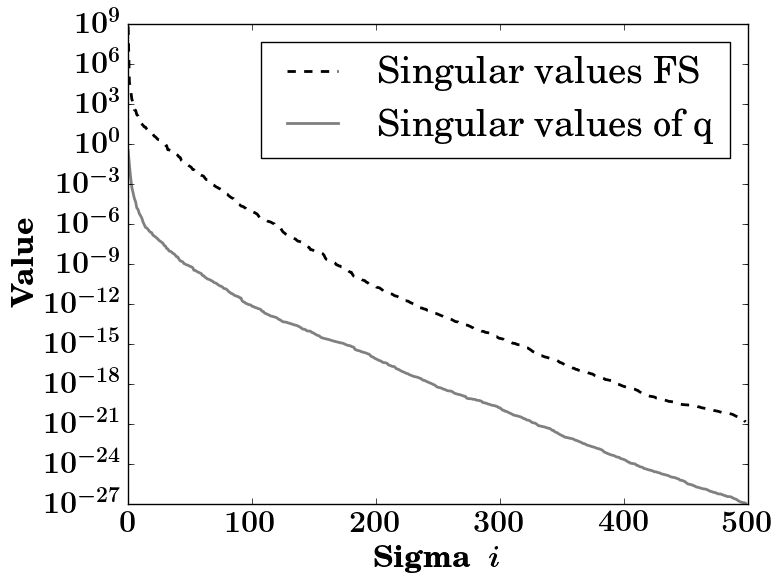
\includegraphics[width=0.6\textwidth]{singularvalues_last_year.png}
  \caption{Distribution of singular values from a SVD of $2880\_1_{3000}$, a matrix of snapshots of a full trajectory of the model year 3000.}
  \label{fig:singularvalues_last_year}
\end{figure}
The relative error of a run with a ROM, created out of the corresponding left singular vectors, over 3000 model years is visible in Figure \ref{fig:error_norm_last_year}.
The ROM $2880\_1_{3000}P150D150$ was initialized with an uniformly distributed concentration of $2.17 \frac{mmol}{m^3}$. The black line shows the relative error to the corresponding model year of the FOM.
The gray dashed line shows the relative error to state of the FOM in the model year 3000. Both are similar, very high and increasing most of the 3000 model years. Thus, starting with a uniformly distribution
does not lead to a usable behavior of the ROM. This is because the POD base projects the initial concentration vector on a low dimensional subspace, i.e. $V^Ty_0 = \hat{y}$, but the vector can not be well approximated in that
subspace.The approximation error $\parallel y_0 - VV^Ty_0 \parallel_2 = 234.3$ is very high. Thus, the initial projection leads to a large error of the ROM. 
\begin{figure}[ht]
\centering
  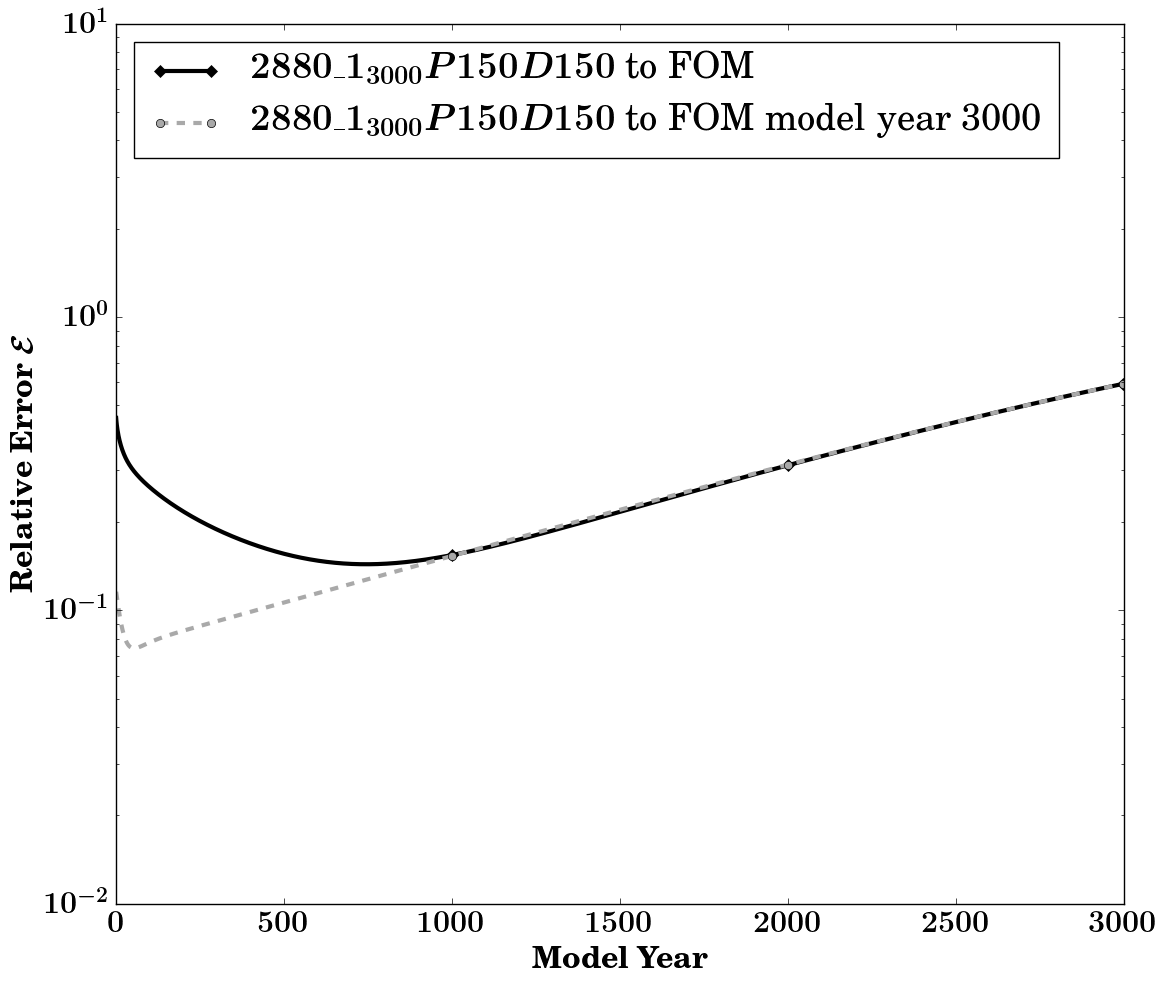
\includegraphics[width=0.8\textwidth]{error_norm_last_year.png}
  \caption[Relative error $\mathcal{E}$ of the reduced-order model $2880\_1_{3000}P150D150$ initialized with an uniformly distributed concentration to the FOM.]{Relative error $\mathcal{E}$ of the reduced-order model $2880\_1_{3000}P150D150$
	    initialized with an uniformly distributed concentration of $2.17 \frac{mmol}{m^3}$ to the FOM. The black line shows the relative error to the corresponding model year of the FOM.
	    The gray dashed line shows the relative error to state of the model year 3000 of the FOM.}
  \label{fig:error_norm_last_year}
\end{figure}
Initializing the ROM with a different concentration, which can be better approximated in the subspace spanned by the POD base, could lead to a better result. Therefore, 
the ROM was initialized with the solution of the FOM in model year 2000. The approximation error $\parallel y_{2000} - VV^Ty_{2000} \parallel_2 = 1.573$ is much smaller.
The relative error to the state of the FOM in model year 3000 is shown by the dashed gray line in Figure \ref{fig:error_norm_last_year_2000}. It is clearly visible that the ROM converges in the first 150 model years to the desired solution and diverges after that. Thus, it would be possible to use the solution of the ROM at that point, where the relative error has its minimum. Since the relative error can only be computed if the original solution is known, it would be more practical to select that point out of other information. 
\begin{figure}[ht]
\centering
  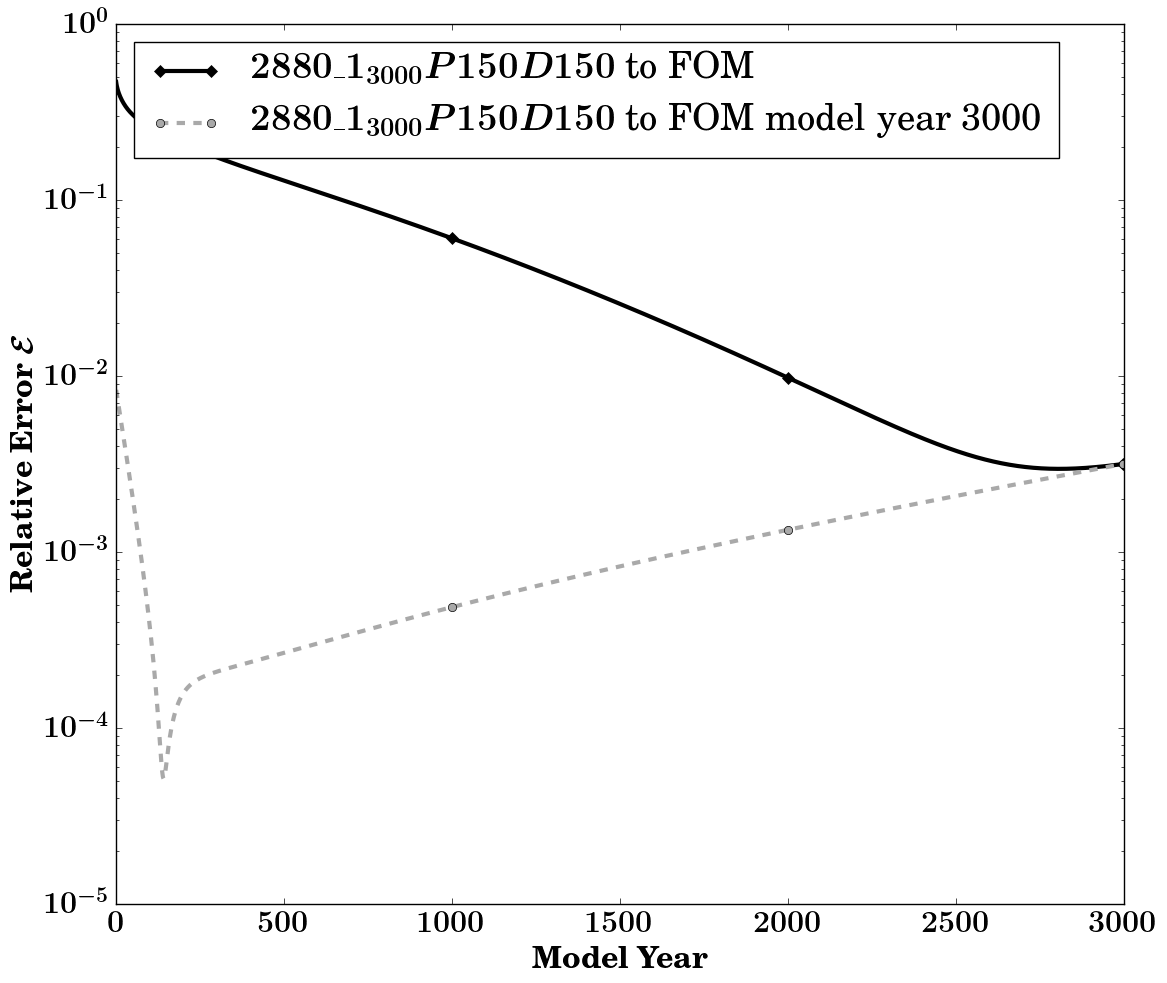
\includegraphics[width=0.8\textwidth]{error_norm_last_year_2000.png}
  \caption[Relative error $\mathcal{E}$ of the reduced-order model $2880\_1_{3000}P150D150$ initialized with the solution of model year 2000 of the FOM.]{Relative error $\mathcal{E}$ of the reduced-order model $2880\_1_{3000}P150D150$
	    initialized with the solution of model year 2000 of the FOM. The black line shows the relative error to the corresponding model year of the FOM.
	    The gray dashed line shows the relative error to state of the model year 3000 of the FOM.}
  \label{fig:error_norm_last_year_2000}
\end{figure}
The spin-up norm of this ROM shows an minimum at that point as well, visible in Figure \ref{fig:spinupnorm_last_year_2000}. It is not exactly the same point but it is quite close. The minimum of the relative error occurs in model year 141 and the minimum of the spin-up norm in model year 231. The information of the spin-up norm could be used to stop the ROM at the right model year to get an usable solution. Thus, a ROM created only with the trajectory of on model year can be used to generate a usable solution. It only has to be initialized with a concentration distribution that is closer to the one of the year the ROM was created with.
\begin{figure}[H]
\centering
  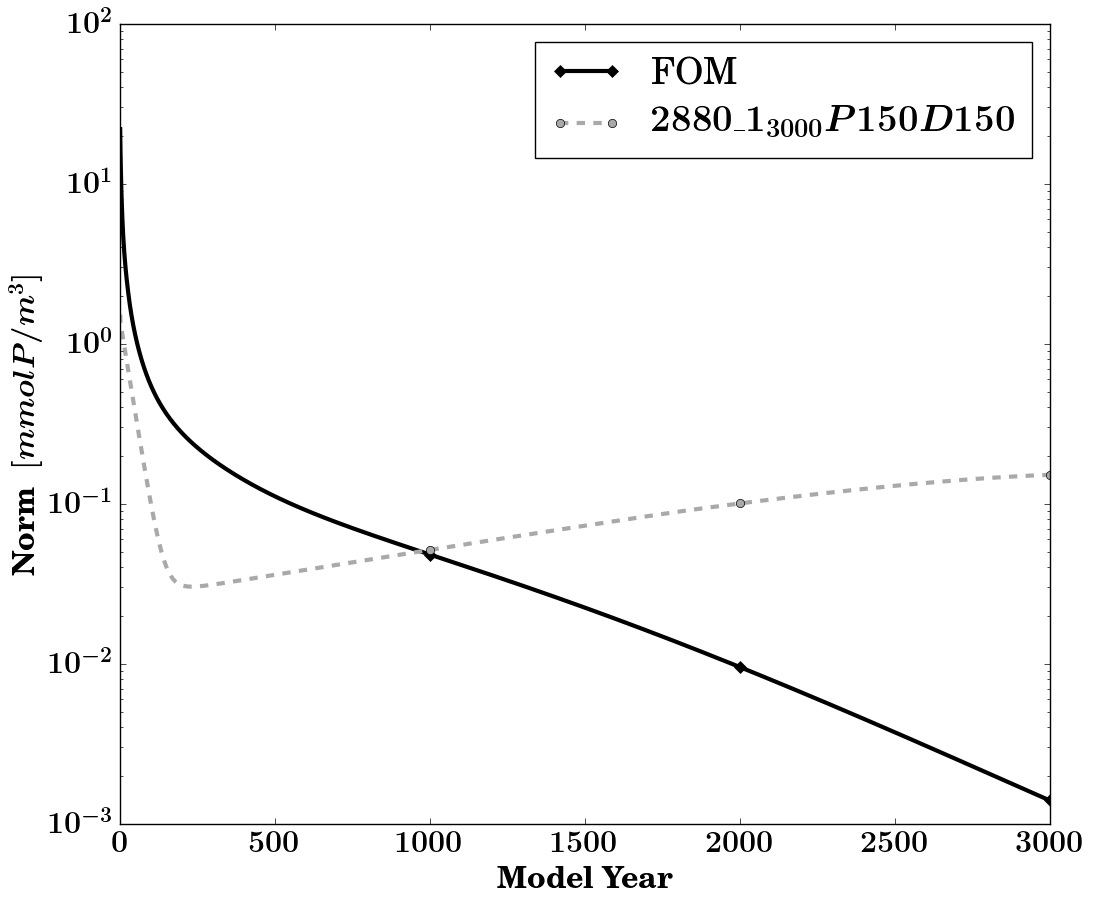
\includegraphics[width=0.8\textwidth]{spinupnorm_last_year_2000.png}
  \caption{Spin-up norm of the reduced-order model $2880\_1_{3000}P150D150$ in comparison with the spin-up norm of the full-order model.}
  \label{fig:spinupnorm_last_year_2000}
\end{figure}


\section{Implementation Issue} % Main appendix title

\label{AppendixA} % For referencing this appendix elsewhere, use \ref{AppendixA}
In the progress of this thesis, tests have shown that there is a small numerical difference in the matrix vector multiplication implemented in numpy and PETSc.
The same matrix vector operation has different results. This difference has been tracked down to the different order in which the addition in the matrix multiplication is performed. There, with some matrices vector combinations 
a difference of $4.44e^{-16}$ occurred, which is double the machine epsilon $\epsilon = 2.22e^{-16}$ for double precision floating point numbers. This happens because floating point additions are not necessarily associative.
In Figure \ref{fig:error_py_m3d} the absolute error between a model run in python and Metos3D is plotted. The example code and data can be found via
\begin{equation*}
 \text{\url{https://github.com/neeljp/matMult_error_python_petsc}.}
\end{equation*}
and can be used for further investigations at any time.

\begin{figure}[H]
\centering
  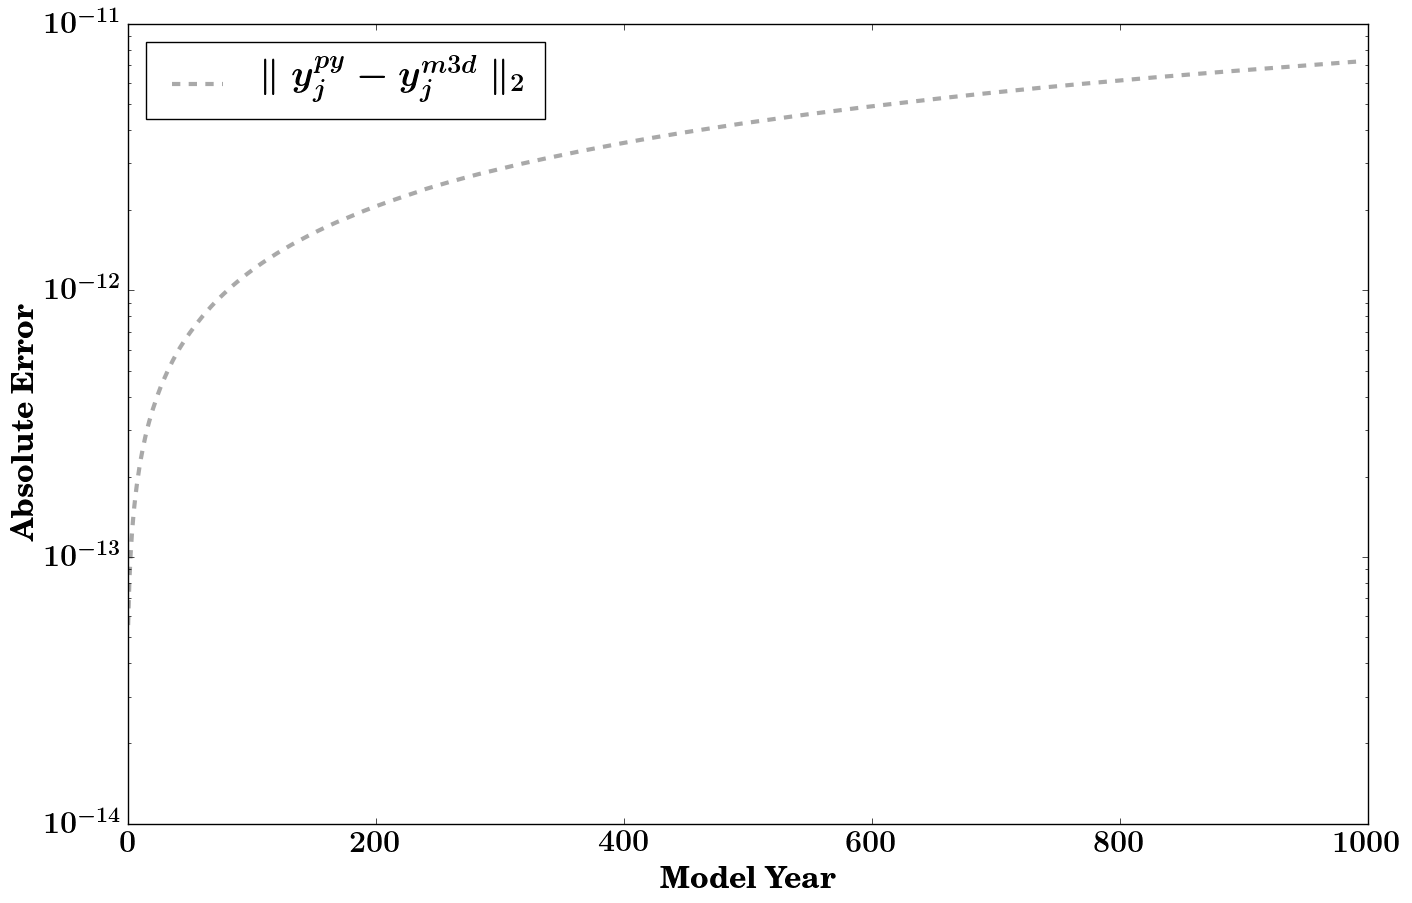
\includegraphics[width=0.9\textwidth]{error_norm_python_petsc.png}
  \caption[Absolute error of a model run with python and with PETSc]{Absolute error $\parallel y^{py}_j - y^{m3d}_j \parallel_2$ of a model run with python and with PETSc over 1000 model years.}
  \label{fig:error_py_m3d}
\end{figure}

\section{Distribution of the CPU time of the main operations of the ROMs} % Main appendix title
\label{Appendix:cpupie}
\begin{figure}[H]
\begin{subfigure}{.40\textwidth}
  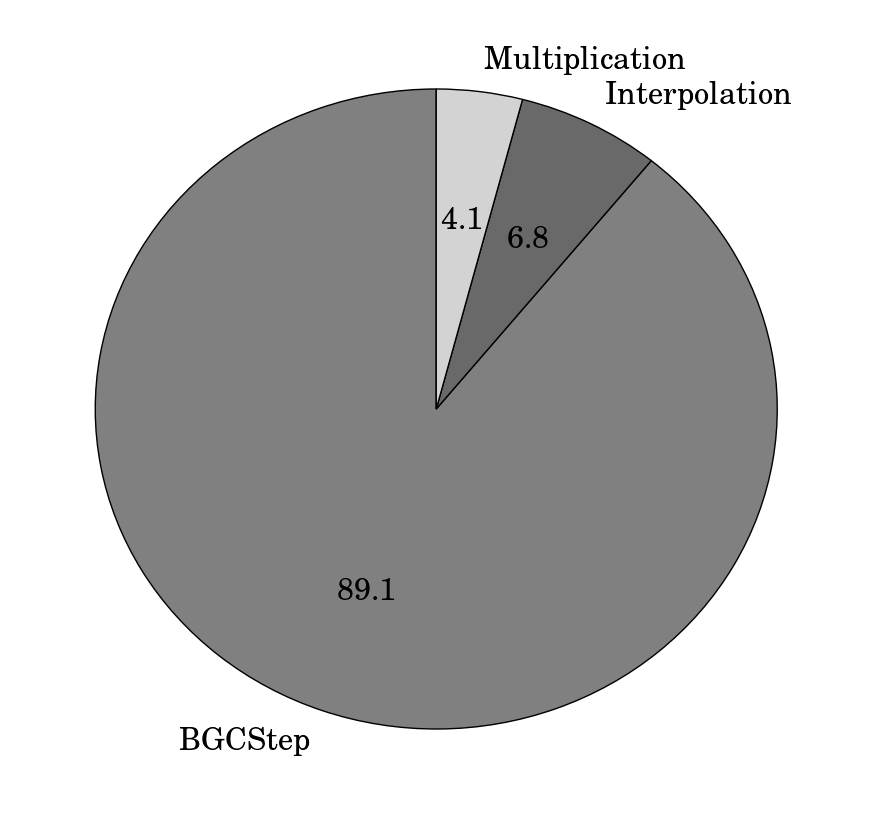
\includegraphics[width=1\textwidth]{timings_P100.png}
  \caption{Base POD100DEIM50}
  \label{fig:timings_sub1}
\end{subfigure}%
\begin{subfigure}{.40\textwidth}
  \centering
  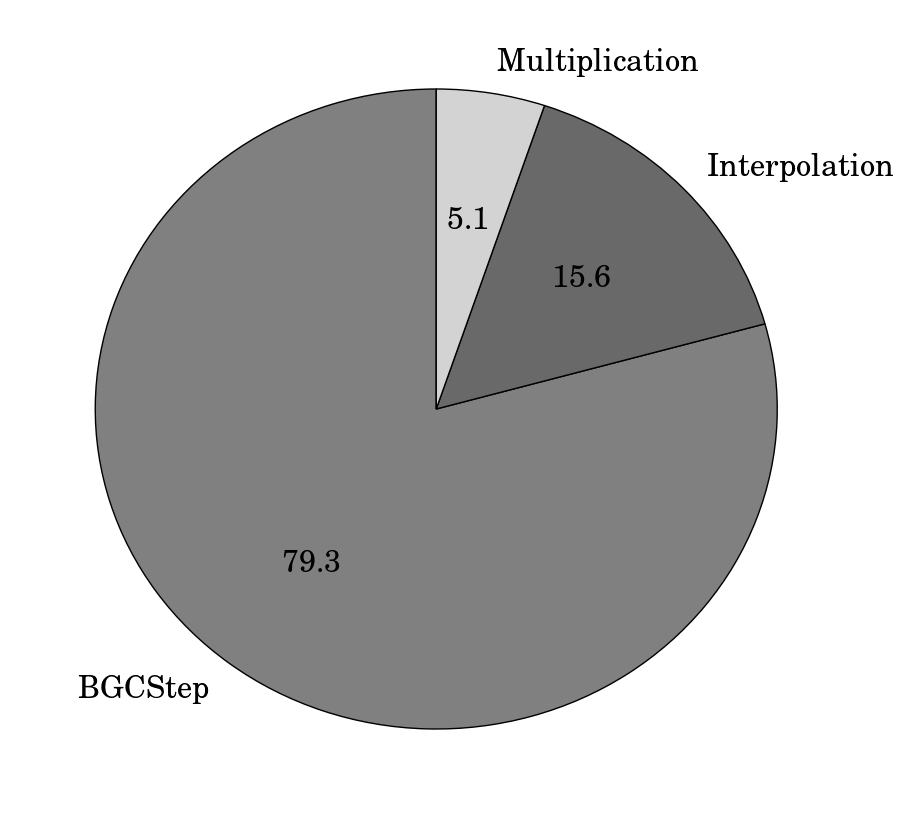
\includegraphics[width=1\textwidth]{timings_P300.png}
  \caption{Base POD300DEIM300}
  \label{fig:timings_sub2}
\end{subfigure}
\caption{Distribution of the computational time among main operations of the N-Model during the computation of a model year. The BGCStep part indicates the time that is needed to evaluate the nonlinear function.}
\label{fig:comparison_timings}
\end{figure}

\begin{figure}[H]
\begin{subfigure}{.48\textwidth}
  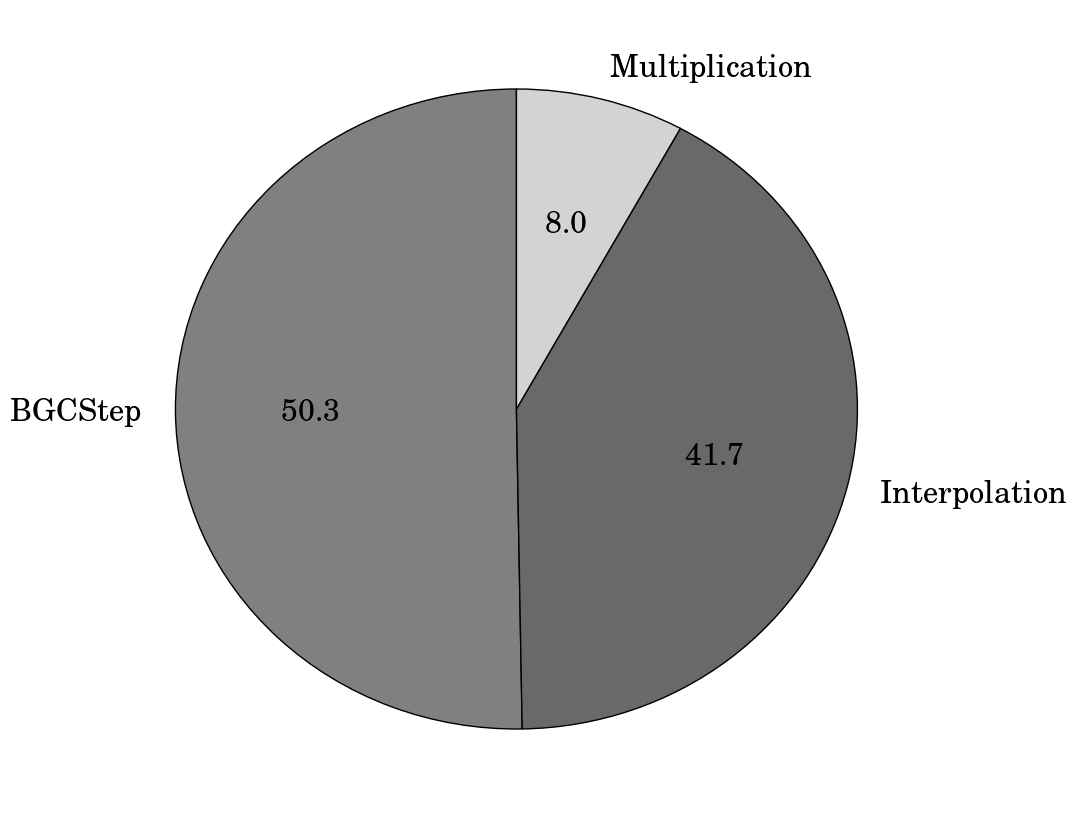
\includegraphics[width=1\textwidth]{timings_P100NDOP.png}
  \caption{Base POD100DEIM50}
  \label{fig:timings_N-DOPsub1}
\end{subfigure}%
\begin{subfigure}{.5\textwidth}
  \centering
  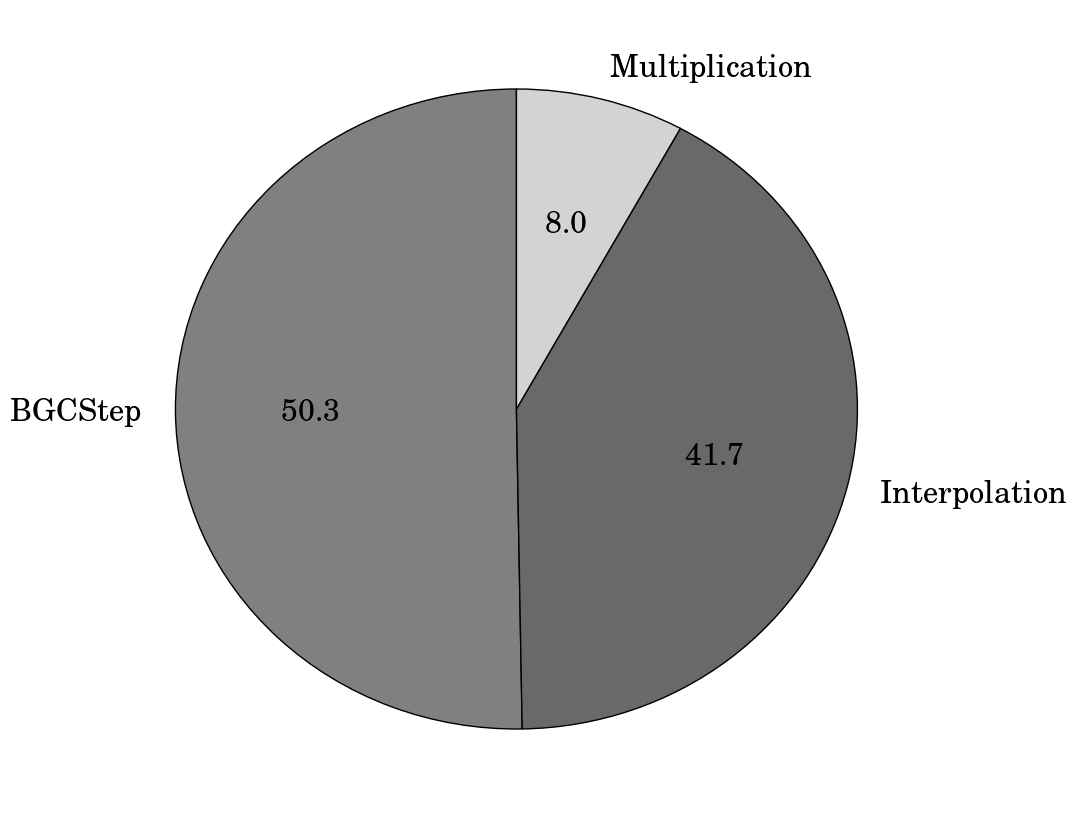
\includegraphics[width=1\textwidth]{timings_P100NDOP.png}
  \caption{Base POD300DEIM300}
  \label{fig:timings_N-DOPsub2}
\end{subfigure}
\caption{Distribution of the computational time among main operations of the N-DOP-Model during the computation of a model year.The BGCStep part indicates the time that is needed to evaluate the nonlinear function.}
\label{fig:comparison_timings_N-DOP}
\end{figure}

\section{Latin Hypercube samples}
\begin{table}[H]
\begin{center} 


$\begin{array}{|l|c|}
\hline
u_{LHC_0} & \{0.0470,140.86,1.305,17.078,0.891\}\\
\hline
u_{LHC_1} & \{0.0254,39.37,0.710,34.632,0.766\}\\
\hline
u_{LHC_2} & \{0.0405,175.83,0.392,19.928,1.251\}\\
\hline
u_{LHC_3} & \{0.0450,137.58,1.154,39.281,1.066\}\\
\hline
u_{LHC_4} & \{0.0289,113.77,0.594,26.857,1.488\}\\
\hline
u_{LHC_5} & \{0.0215,184.91,0.294,45.932,1.321\}\\
\hline
u_{LHC_6} & \{0.0332,58.38,1.473,24.204,1.363\}\\
\hline
u_{LHC_7} & \{0.0373,98.79,1.052,11.707,1.133\}\\
\hline
u_{LHC_8} & \{0.0121,63.83,0.787,46.016,0.828\}\\
\hline
u_{LHC_9} & \{0.0162,14.21,0.933,30.877,0.959\}\\
\hline
\end{array}$
\end{center}
\caption{10 Latin Hypercube samples used in Chapter \ref{Chapter5}.}
 \label{Chapter5:table_lhc_sample}
\end{table}

\section{Plots of parametrized models}

\begin{figure}[H]
\centering
  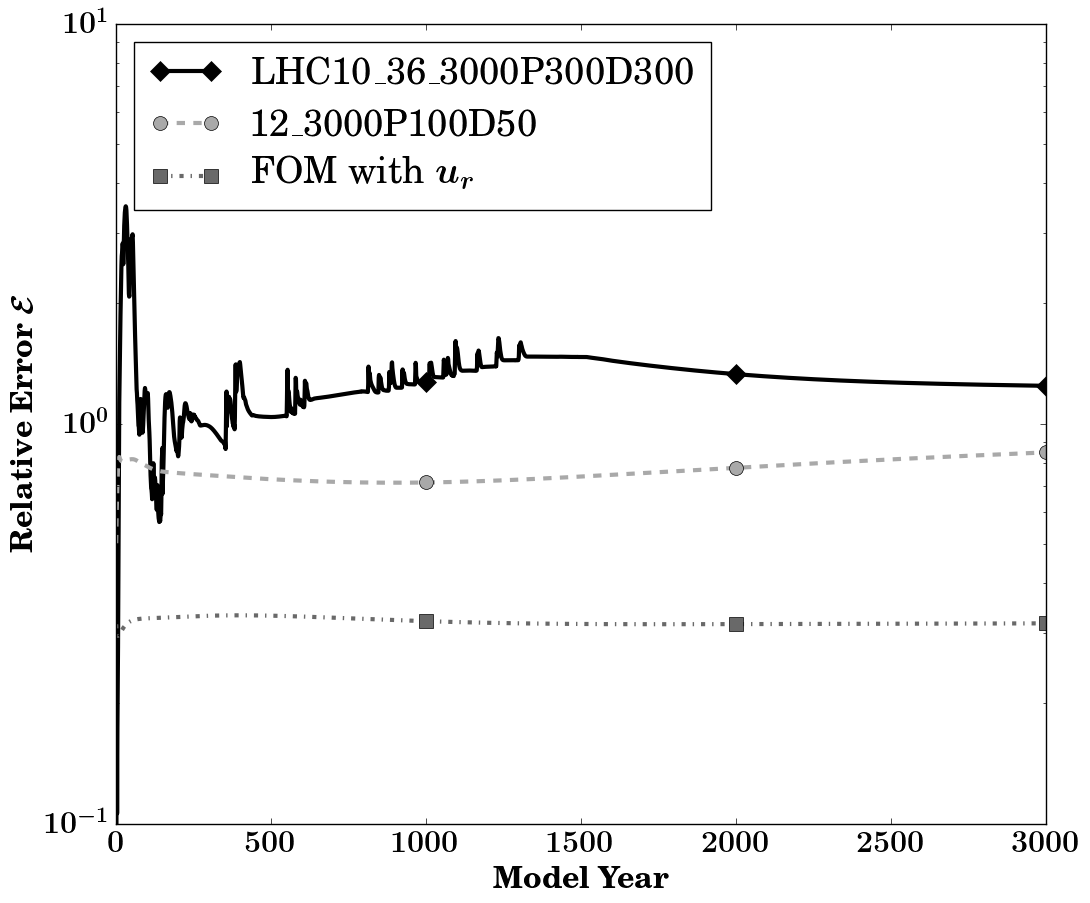
\includegraphics[width=0.9\textwidth]{error_norm_lhc_0.png}
  \captionsetup{width=1\textwidth}
  \caption[Relative error between different model runs and the FOM solution generated with $u_{LHC_0}$.]{Relative error between different model runs and the FOM solution generated with $u_{LHC_0}$. The black line is the relative error of the ROM generated with the
  ten Hypercube samples, run with $u_{LHC_0}$. The gray line with dots shows the relative error of the ROM out of Chapter 4 generated with the parameters set $u_r$, run with $u_{LHC_0}$.
  The dotted line with squares represents the relative error to the original solution of the FOM, run with parameter set $u_r$.}
  \label{fig:error_norm_lhc_0}
\end{figure}

\begin{figure}[H]
\centering
  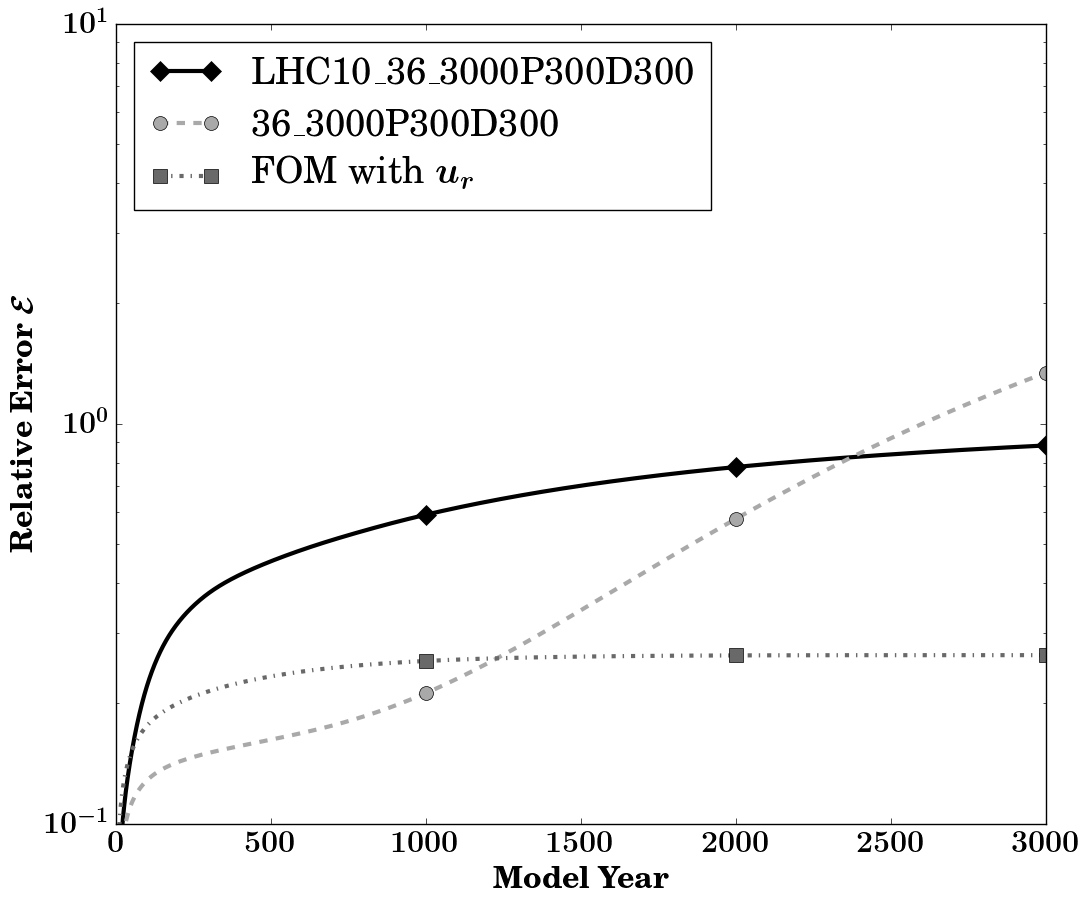
\includegraphics[width=0.9\textwidth]{error_norm_+50.png}
  \captionsetup{width=1\textwidth}
  \caption[Relative error between different model runs and the FOM solution generated with $u_r + 50\%$.]{Relative error between different model runs and the FOM solution generated with $u_r + 50\%$. The black line is the relative error of the ROM generated with the
  ten Hypercube samples, run with $u_r + 50\%$. The gray line with dots shows the relative error of the ROM $36\_3000P300D300$ out of Chapter 4 generated with the parameters set $u_r$, run with  $u_r + 50\%$.
  The dotted line with squares represents the relative error to the original solution of the FOM, run with parameter set $u_r$.}
  \label{fig:error_norm_+50}
\end{figure}

